\documentclass{article}

% Formato base: talleres/Homework_3_PIC.pdf (article 10 pt, carta, Computer/Latin Modern).
% Compilar con XeLaTeX o Tectonic:  tectonic Tarea_1_ONL.tex
\usepackage[spanish,es-tabla,es-nodecimaldot]{babel}
\usepackage{fontspec}
\usepackage{amsmath,amssymb,mathtools}
\usepackage{cancel}
\usepackage{graphicx}
\usepackage{booktabs}
\usepackage{siunitx}
\usepackage{xcolor}
\usepackage{float}
\usepackage{pgfplots}
\pgfplotsset{compat=1.17}
\usetikzlibrary{babel}
\usepackage{hyperref}

\sisetup{output-decimal-marker={.}, per-mode=symbol}
\hypersetup{colorlinks=true, linkcolor=black, citecolor=black, urlcolor=black}

% Notación de Saleh: campos reales en caligráfica, amplitudes complejas en negrita.
\newcommand{\Ec}{\boldsymbol{\mathcal{E}}}
\newcommand{\Hc}{\boldsymbol{\mathcal{H}}}
\newcommand{\Pc}{\boldsymbol{\mathcal{P}}}
\newcommand{\Pe}{\mathcal{P}}
\newcommand{\Ee}{\mathcal{E}}
\newcommand{\VT}{V_T}
\newcommand{\dd}{\,\mathrm{d}}
\newcommand{\xh}{\hat{\mathbf{x}}}
\newcommand{\yh}{\hat{\mathbf{y}}}
\newcommand{\zh}{\hat{\mathbf{z}}}
\newcommand{\env}{e^{-\frac{(t-z/c_0)^2}{\tau^2}}}

\title{Tarea 1}
\author{Juan E. Rodriguez Ochoa\\
Profesor: Rodrigo Acuña Herrera\\
Óptica No Lineal, Escuela de Física\\
Universidad Nacional de Colombia, Sede Medellín}
\date{Septiembre 2026}

\begin{document}
\maketitle

\noindent\textbf{Convenciones.} Se usan unidades SI y la notación de Saleh y Teich (\emph{Fundamentals of Photonics}, 2.ª ed.): los
campos reales se escriben $\Ec(\mathbf r,t)$, $\Hc(\mathbf r,t)$, las amplitudes complejas
$\mathbf E(\mathbf r)$, $\mathbf H(\mathbf r)$, la dependencia temporal es $e^{j\omega t}$ y
$j=\sqrt{-1}$ (en los puntos 2 y 3, además, $j$ evita confundir la unidad imaginaria con la
corriente $i$). Las constantes usadas son $c_0=\SI{2.998e8}{m/s}$,
$\epsilon_0=\SI{8.854e-12}{F/m}$, $\mu_0=4\pi\times10^{-7}\,\mathrm{H/m}$ y
$\eta_0=\sqrt{\mu_0/\epsilon_0}\approx\SI{377}{\ohm}$.

%=====================================================================
\section{Punto 1: Onda electromagnética con envolvente gaussiana}
%=====================================================================

\emph{Una onda electromagnética en el espacio libre tiene el vector de campo eléctrico
$\Ec=f(t-z/c_0)\,\xh$, donde $f(t)=\exp(-t^2/\tau^2)\exp(j2\pi\nu_0t)$ y $\tau$ es una constante.
Describa la naturaleza física de la onda y determine una expresión para el vector de campo
magnético} (Saleh y Teich, ejercicio 5.1-1, p.~195).

\bigskip

\[
\Ec=f\!\left(t-\frac{z}{c_0}\right)\xh,\qquad f(t)=e^{-\frac{t^2}{\tau^2}}\,e^{j2\pi\nu_0t},
\qquad\text{con }\tau\text{ una constante.}
\]

Reemplazando $f(t)$ en $\Ec(z,t)$:
\[
\Ec=e^{-\frac{(t-z/c_0)^2}{\tau^2}}\,e^{j2\pi\nu_0(t-z/c_0)}\,\xh
\]
\[
\Ec=e^{-\frac{(t-z/c_0)^2}{\tau^2}}\,e^{j\omega_0t}\,e^{-jk_0z}\,\xh,
\qquad \omega_0=2\pi\nu_0,\quad k_0=\frac{\omega_0}{c_0}.
\]

La última expresión representa el vector de campo eléctrico con un pulso envolvente temporal y
espacial gaussiano, con polarización lineal en dirección horizontal (eje $x$), siguiendo el
marco de referencia de la figura~\ref{fig:p1}. De la expresión se leen las demás características
de la onda:
\begin{itemize}
  \item \textbf{Dirección de propagación:} el campo depende de $z$ y $t$ solo a través de
  $t-z/c_0$, así que el pulso viaja sin deformarse en la dirección $+z$ con velocidad $c_0$.
  \item \textbf{Envolvente:} $\exp[-(t-z/c_0)^2/\tau^2]$, un pulso gaussiano de duración del
  orden de $\tau$ en el tiempo y de extensión del orden de $c_0\tau$ en el espacio.
  \item \textbf{Factor de propagación (portadora):} $e^{j(\omega_0t-k_0z)}$, una onda plana de
  frecuencia $\nu_0$ y número de onda $k_0=\omega_0/c_0=2\pi/\lambda_0$. El campo físico es la
  parte real, $\mathrm{Re}\{\Ec\}$.
  \item \textbf{Polarización:} lineal, siempre a lo largo de $\xh$.
\end{itemize}

\begin{figure}[H]
\centering
\begin{tikzpicture}
\begin{axis}[
  width=0.85\textwidth, height=5.2cm,
  xlabel={Posición relativa al centro del pulso, $(z-c_0t)/(c_0\tau)$ (adimensional)},
  ylabel={$\mathrm{Re}\{\mathcal{E}_x\}$ (unid. arb.)},
  xmin=-3, xmax=3, ymin=-1.25, ymax=1.35, samples=600, domain=-3:3,
  axis lines=left, grid=major, grid style={black!10},
  legend style={at={(0.99,0.99)}, anchor=north east, font=\footnotesize, draw=none, fill=white, fill opacity=0.85},
  label style={font=\small}, tick label style={font=\footnotesize}]
  \addplot[red!75!black, thick] {exp(-x^2)*cos(deg(2*pi*3*x))};
  \addlegendentry{campo $\mathcal{E}_x$ (portadora)}
  \addplot[black, dashed] {exp(-x^2)};
  \addlegendentry{envolvente gaussiana}
  \addplot[black, dashed, forget plot] {-exp(-x^2)};
  \draw[->, very thick, blue!60!black] (axis cs:-2.8,1.05) -- (axis cs:-1.7,1.05)
    node[right, font=\small] {$\mathbf{k}_0\parallel+\hat{\mathbf z}$};
\end{axis}
\end{tikzpicture}
\caption{Instantánea del campo eléctrico del punto 1 a lo largo del eje de propagación, para un
valor ilustrativo $\nu_0\tau=3$ (en el óptico $\nu_0\tau\gg1$ y hay muchos más ciclos bajo la
envolvente). El campo oscila a lo largo de $\hat{\mathbf x}$ y el pulso completo avanza en $+z$ con
velocidad $c_0$.}
\label{fig:p1}
\end{figure}

Veamos una expresión del campo magnético usando la ley de Faraday (Saleh y Teich, ec.~(5.1-8), p.~154)
(en el espacio libre $\mathcal{B}=\mu_0\mathcal{H}$):
\[
\nabla\times\Ec=-\mu_0\frac{\partial\Hc}{\partial t},
\qquad
\nabla\times\Ec=
\begin{vmatrix}
\xh & \yh & \zh\\[2pt]
\dfrac{\partial}{\partial x} & \dfrac{\partial}{\partial y} & \dfrac{\partial}{\partial z}\\[8pt]
\env e^{j\omega_0t}e^{-jk_0z} & 0 & 0
\end{vmatrix}.
\]
Como $\Ec$ solo tiene componente $x$ y solo depende de $z$ y $t$, el único término que sobrevive es
\[
\nabla\times\Ec=\frac{\partial}{\partial z}\left(\env e^{j\omega_0t}e^{-jk_0z}\right)\yh .
\]
Derivando el producto, con la regla de la cadena para la envolvente,
\[
\frac{\partial}{\partial z}\env=\env\left[-\frac{2(t-z/c_0)}{\tau^2}\right]\left(-\frac{1}{c_0}\right)
=\frac{2(t-z/c_0)}{\tau^2c_0}\env ,
\]
se obtiene
\[
=\left(\frac{2(t-z/c_0)}{\tau^2c_0}\,\env e^{j\omega_0t}e^{-jk_0z}-jk_0\,\mathcal{E}_x(z,t)\right)\yh
\]
\[
=\left(\frac{2(t-z/c_0)}{\tau^2c_0}-jk_0\right)\env e^{j\omega_0t}e^{-jk_0z}\,\yh
=-\mu_0\frac{\partial\Hc}{\partial t}.
\]

Integramos temporalmente, desde $-\infty$ (donde el pulso aún no ha llegado y los campos son
nulos, así que no hay constante de integración) hasta $t$:
\[
-\mu_0\Hc=\int_{-\infty}^{t}\left(\frac{2(t'-z/c_0)}{\tau^2c_0}-jk_0\right)
e^{-\frac{(t'-z/c_0)^2}{\tau^2}}e^{j\omega_0t'}e^{-jk_0z}\,\yh\dd t'
\]
\begin{multline*}
=\Bigg[\frac{2}{\tau^2c_0}e^{-jk_0z}\int_{-\infty}^{t}\left(t'-\frac{z}{c_0}\right)
e^{-\frac{(t'-z/c_0)^2}{\tau^2}}e^{j\omega_0t'}\dd t'\\
-jk_0e^{-jk_0z}\int_{-\infty}^{t}e^{-\frac{(t'-z/c_0)^2}{\tau^2}}e^{j\omega_0t'}\dd t'\Bigg]\yh .
\end{multline*}
Para abreviar se llama $\displaystyle\mathcal{J}(z,t)\equiv\int_{-\infty}^{t}e^{-\frac{(t'-z/c_0)^2}{\tau^2}}e^{j\omega_0t'}\dd t'$
a la integral que se repite. La primera integral se hace por partes, con $u=e^{j\omega_0t'}$ y
$\dd v=(t'-z/c_0)\,e^{-(t'-z/c_0)^2/\tau^2}\dd t'$, de modo que
$v=-\frac{\tau^2}{2}e^{-(t'-z/c_0)^2/\tau^2}$ (el término de borde en $-\infty$ se anula):
\[
=\left[\frac{2}{\tau^2c_0}e^{-jk_0z}\left(-e^{j\omega_0t}\frac{\tau^2}{2}\env
+\frac{j\omega_0\tau^2}{2}\,\mathcal{J}\right)
-jk_0e^{-jk_0z}\,\mathcal{J}\right]\yh
\]
\[
=\left[-\frac{1}{c_0}\env e^{-jk_0z}e^{j\omega_0t}
+\frac{j\omega_0}{c_0}e^{-jk_0z}\,\mathcal{J}
-jk_0e^{-jk_0z}\,\mathcal{J}\right]\yh .
\]
Y como $\omega_0/c_0=k_0$, luego los dos últimos términos se cancelan:
\[
=\left[-\frac{1}{c_0}\env e^{-jk_0z}e^{j\omega_0t}
+\cancel{\frac{j\omega_0}{c_0}e^{-jk_0z}\,\mathcal{J}}
-\cancel{jk_0e^{-jk_0z}\,\mathcal{J}}\right]\yh .
\]
Al final:
\[
-\mu_0\Hc(z,t)=-\frac{1}{c_0}\env e^{-jk_0z}e^{j\omega_0t}\,\yh
\]
\[
\boxed{\;\Hc(z,t)=\frac{1}{\mu_0c_0}\,e^{-\frac{(t-z/c_0)^2}{\tau^2}}\,e^{-jk_0z}\,e^{j\omega_0t}\,\yh
=\frac{1}{\eta_0}\,f\!\left(t-\frac{z}{c_0}\right)\yh\;}
\]
donde se usó $\mu_0c_0=\mu_0/\sqrt{\epsilon_0\mu_0}=\sqrt{\mu_0/\epsilon_0}=\eta_0$. Al final se
cumple la dirección de propagación con las direcciones de $\Ec$ y $\Hc$: $\Ec\parallel\xh$,
$\Hc\parallel\yh$ y $\xh\times\yh=\zh$, que es justamente la dirección en que viaja el pulso. Además
$|\Ec|/|\Hc|=\eta_0$, la misma relación de una onda plana TEM en el espacio libre
(Saleh y Teich, ec.~(5.4-5), p.~165).

%=====================================================================
\newpage
\section{Punto 2: Espectro de salida de sistemas no lineales}
%=====================================================================

\emph{Use MATLAB para dibujar la amplitud de la transformada de Fourier de la salida versus
frecuencia de los siguientes sistemas y entradas: (a) dispositivo con la ley $i=v^2$ con entrada
$v=\cos(2\pi50t)+\cos(2\pi120t)$; (b) un diodo mezclador con función de transferencia
$i=i_0[\exp(ev/kT)-1]$, donde $i_0=\SI{10}{pA}$ es la corriente de polarización inversa y
$kT/e=\SI{26}{mV}$ a temperatura ambiente. La entrada es $v=0.3+0.2\cos(2\pi50t)$, en voltios.}

\subsection*{¿Por qué un sistema no lineal crea frecuencias nuevas?}

Un sistema lineal solo puede cambiar la amplitud y la fase de cada frecuencia de entrada: si entra
$\cos\omega t$, sale $A\cos(\omega t+\varphi)$. Un sistema no lineal sin memoria aplica una función
$g$ al valor instantáneo de la entrada, $i(t)=g(v(t))$. Si $g$ contiene potencias $v^n$, al elevar un
coseno a una potencia aparecen cosenos de frecuencias múltiplos y, si hay varias frecuencias,
combinaciones de ellas. Es la misma física de la óptica no lineal, donde la polarización se expande
como (Boyd, ec.~(1.1.2), p.~2)
\[
\tilde P(t)=\epsilon_0\left[\chi^{(1)}\tilde E(t)+\chi^{(2)}\tilde E^2(t)+\chi^{(3)}\tilde E^3(t)+\cdots\right].
\]
Aquí el ``campo'' es el voltaje $v$ y la ``polarización'' es la corriente $i$. Las identidades que
se usarán salen de $\cos\alpha=\tfrac12(e^{j\alpha}+e^{-j\alpha})$:
\begin{gather*}
\cos^2\alpha=\tfrac12(1+\cos2\alpha),\qquad
\cos^3\alpha=\tfrac14(3\cos\alpha+\cos3\alpha),\\
\cos\alpha\cos\beta=\tfrac12[\cos(\alpha-\beta)+\cos(\alpha+\beta)].
\end{gather*}
Por ejemplo, $\cos^3\alpha=\tfrac18(e^{j\alpha}+e^{-j\alpha})^3
=\tfrac18(e^{3j\alpha}+3e^{j\alpha}+3e^{-j\alpha}+e^{-3j\alpha})=\tfrac14\cos3\alpha+\tfrac34\cos\alpha$,
la misma identidad que usa Boyd para el tercer armónico (ec.~(1.2.13), p.~11).

\subsection{Punto 2a: dispositivo de ley cuadrática}

\[
i(t)=v^2(t),\qquad v(t)=\cos\alpha+\cos\beta,\qquad \alpha=2\pi f_1t,\ \beta=2\pi f_2t,
\]
con $f_1=\SI{50}{Hz}$ y $f_2=\SI{120}{Hz}$. El enunciado no da coeficiente, así que se toma
$i=kv^2$ con $k=\SI{1}{A/V^2}$ (con otro $k$ el espectro solo se escala). Desarrollando el cuadrado y
linealizando cada término:
\begin{align*}
i&=\cos^2\alpha+2\cos\alpha\cos\beta+\cos^2\beta\\
&=\tfrac12+\tfrac12\cos2\alpha+\cos(\beta-\alpha)+\cos(\alpha+\beta)+\tfrac12+\tfrac12\cos2\beta ,
\end{align*}
\[
\boxed{\;i(t)=1+\cos(2\pi\,70\,t)+\tfrac12\cos(2\pi\,100\,t)+\cos(2\pi\,170\,t)+\tfrac12\cos(2\pi\,240\,t)\;}
\]
El resultado es exacto: $v^2$ es un polinomio de grado 2 y la salida tiene un número finito de líneas.
Si en Boyd se toma $\tilde E=E_1e^{-j\omega_1t}+E_2e^{-j\omega_2t}+\text{c.c.}$ y se calcula
$\epsilon_0\chi^{(2)}\tilde E^2$, aparecen exactamente los mismos términos
(Boyd, ecs.~(1.2.3)--(1.2.5), p.~6) (tabla~\ref{tab:2a}).

\begin{table}[H]
\centering
\caption{Componentes de la salida del dispositivo cuadrático: predicción analítica, resultado de la
FFT y proceso óptico análogo.}
\label{tab:2a}
\small
\begin{tabular}{@{}ccccl@{}}
\toprule
$f$ (Hz) & Origen & Analítico (A) & FFT (A) & Proceso análogo en óptica no lineal \\
\midrule
0   & $\tfrac12+\tfrac12$ & 1   & 1.000000 & Rectificación óptica (OR) \\
70  & $f_2-f_1$           & 1   & 1.000000 & Diferencia de frecuencias (DFG) \\
100 & $2f_1$              & 0.5 & 0.500000 & Segundo armónico (SHG) \\
170 & $f_1+f_2$           & 1   & 1.000000 & Suma de frecuencias (SFG) \\
240 & $2f_2$              & 0.5 & 0.500000 & Segundo armónico (SHG) \\
\bottomrule
\end{tabular}
\end{table}

Observaciones:
\begin{itemize}
  \item Las frecuencias de entrada (50 y \SI{120}{Hz}) no aparecen en la salida: el término
  cuadrático solo produce sumas y diferencias de pares de frecuencias; para reproducir la entrada
  haría falta un término lineal.
  \item Los productos cruzados pesan el doble que los armónicos (1 frente a 0.5) por el factor 2 de
  $2\cos\alpha\cos\beta$; en Boyd, SFG y DFG llevan $2\chi^{(2)}E_1E_2$ y SHG lleva $\chi^{(2)}E_1^2$.
  \item La salida es periódica con periodo $1/\gcd(50,120)=\SI{0.1}{s}$, así que $T=\SI{1}{s}$
  contiene exactamente 10 periodos.
  \item Parseval: $\langle i^2\rangle=A_0^2+\tfrac12\sum_{k\ge1}A_k^2=1+\tfrac12(1+1+0.25+0.25)=2.25$;
  el promedio numérico de $i^2(t)$ en MATLAB da $2.250000$.
\end{itemize}

\begin{figure}[H]
\centering
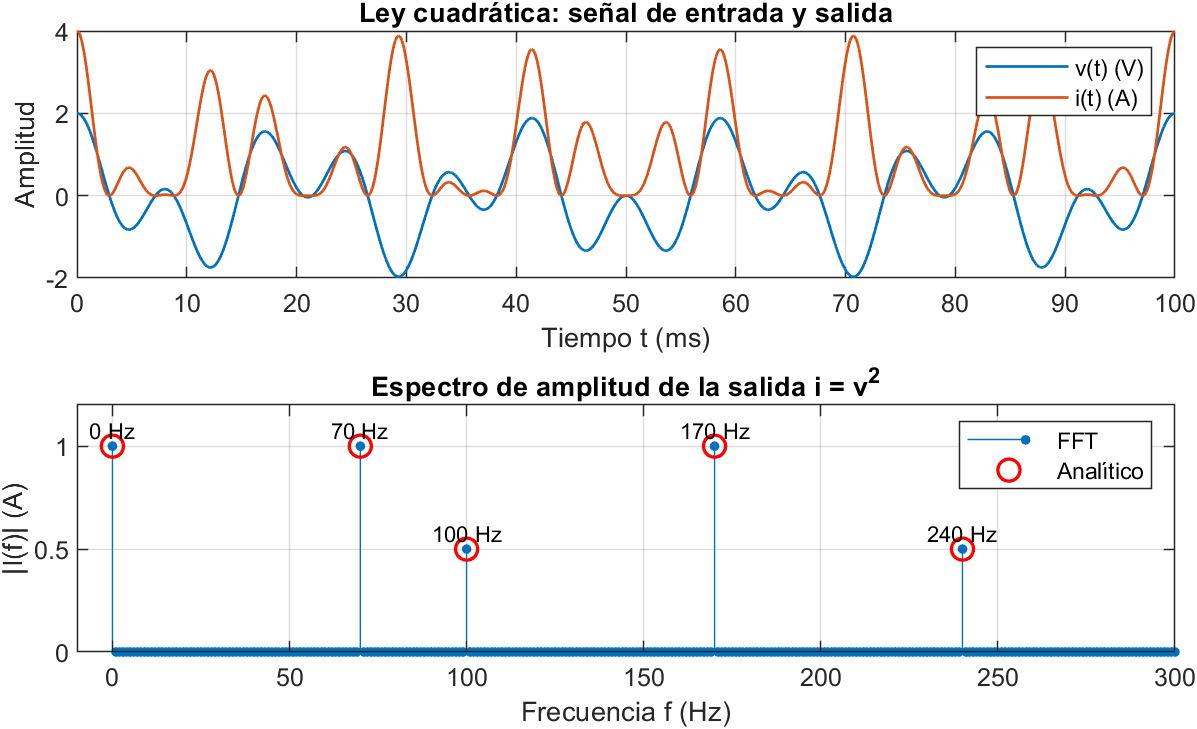
\includegraphics[width=0.95\textwidth]{figuras/punto2a_espectro.png}
\caption{Punto 2a. Arriba: entrada $v(t)$ y salida $i(t)=v^2$ en los primeros \SI{100}{ms} (un periodo
de la salida). Abajo: amplitud del espectro de la salida calculada con la FFT (azul) y predicción
analítica (círculos rojos).}
\label{fig:2a}
\end{figure}

\subsection{Punto 2b: diodo mezclador}

Se usa la ecuación de Shockley del diodo,
\[
i=i_0\left[\exp\!\left(\frac{ev}{kT}\right)-1\right]=i_0\left[e^{v/\VT}-1\right],\qquad
\VT\equiv\frac{kT}{e}=\SI{26}{mV},
\]
donde $\VT$ es el voltaje térmico, la escala de voltaje en la que la exponencial cambia
apreciablemente. La entrada es $v(t)=V_0+V_1\cos\omega t$ con $V_0=\SI{0.3}{V}$, $V_1=\SI{0.2}{V}$ y
$f=\SI{50}{Hz}$.

\textbf{Nota sobre el enunciado.} El enunciado escribe $i=i_0[\exp(ev/kT-1)]$, con el $-1$ dentro de
la exponencial. Se tomó como error de digitación y se usó la forma de Shockley por tres razones: con
$v=0$ debe ser $i=0$ (la forma literal da $i_0/e\approx\SI{3.7}{pA}$); $i_0$ se llama corriente de
polarización inversa, y solo con Shockley $i\to-i_0$ en inversa fuerte; y es la ecuación estándar del
diodo. Si se tomara literal, $i=(i_0/e)\,e^{v/\VT}$: el espectro es el mismo escalado por
$1/e\approx0.368$ (DC \SI{0.1211}{mA}, \SI{50}{Hz} \SI{0.2258}{mA}, \SI{100}{Hz} \SI{0.1834}{mA},
\SI{150}{Hz} \SI{0.1304}{mA}) y el resultado del punto 3 no cambia, porque el factor constante se
cancela en la razón.

\textbf{Paso 1: separar la polarización.} Como $e^{a+b}=e^ae^b$,
\[
i(t)=i_0e^{V_0/\VT}e^{(V_1/\VT)\cos\omega t}-i_0=I_s\,e^{x\cos\omega t}-i_0,
\]
\[
I_s\equiv i_0e^{V_0/\VT}=(\SI{10}{pA})\,e^{11.538}=\SI{1.0259}{\micro A},\qquad
x\equiv\frac{V_1}{\VT}=\frac{\SI{0.2}{V}}{\SI{0.026}{V}}=7.6923 .
\]
$I_s$ es la corriente en el punto de operación y $x$ mide qué tan grande es la señal frente a la escala
de la no linealidad.

\textbf{Paso 2: serie de Fourier de $e^{x\cos\theta}$.} Se parte de la función generatriz de las
funciones de Bessel modificadas:
\begin{align*}
\exp\!\left[\frac x2\left(t+\frac1t\right)\right]
&=\left(\sum_{m=0}^{\infty}\frac{(x/2)^mt^m}{m!}\right)\left(\sum_{k=0}^{\infty}\frac{(x/2)^kt^{-k}}{k!}\right)
=\sum_{n=-\infty}^{\infty}I_n(x)\,t^n,\\
I_n(x)&=\sum_{k=0}^{\infty}\frac{(x/2)^{2k+n}}{k!\,(k+n)!},
\end{align*}
donde se agruparon las potencias $t^n$ ($m=n+k$) y se reconoció la serie de la función de Bessel
modificada de primera especie, con $I_{-n}=I_n$. Tomando $t=e^{j\theta}$, de modo que
$\tfrac12(t+1/t)=\cos\theta$:
\[
e^{x\cos\theta}=I_0(x)+\sum_{n=1}^{\infty}I_n(x)\left(e^{jn\theta}+e^{-jn\theta}\right)
=I_0(x)+2\sum_{n=1}^{\infty}I_n(x)\cos n\theta .
\]

\textbf{Paso 3: la salida exacta.} Con $\theta=\omega t$,
\[
\boxed{\;i(t)=\big[I_sI_0(x)-i_0\big]+\sum_{n=1}^{\infty}2I_sI_n(x)\cos(2\pi\,n\,50\,t)\;}
\]
La salida contiene DC y todos los armónicos de \SI{50}{Hz}, con amplitud
$A_n=2I_sI_n(x)$; en MATLAB, $I_n(x)$ se evalúa con \texttt{besseli(n,x)}. Por ejemplo, $A_1=2(\SI{1.0259}{\micro A})(299.136)=\SI{0.6137}{mA}$ y
$A_0=(\SI{1.0259}{\micro A})(320.778)-\SI{10}{pA}=\SI{0.3291}{mA}$.

\begin{table}[H]
\centering
\caption{Punto 2b: $I_n(x)$ para $x=7.6923$ y amplitudes de la corriente, por Bessel y por FFT
(\texttt{punto2b.m}).}
\label{tab:2b}
\small
\begin{tabular}{@{}cccccc@{}}
\toprule
$n$ & $f$ (Hz) & $I_n(x)$ & $|I|$ Bessel (mA) & $|I|$ FFT (mA) & $A_n/A_1$ \\
\midrule
0 & 0   & 320.778 & 0.329075 & 0.329075 & 0.536 \\
1 & 50  & 299.136 & 0.613746 & 0.613746 & 1.000 \\
2 & 100 & 243.003 & 0.498576 & 0.498576 & 0.812 \\
3 & 150 & 172.775 & 0.354487 & 0.354487 & 0.578 \\
4 & 200 & 108.239 & 0.222076 & 0.222076 & 0.362 \\
5 & 250 & 60.207  & 0.123528 & 0.123528 & 0.201 \\
6 & 300 & 29.970  & 0.061490 & 0.061490 & 0.100 \\
7 & 350 & 13.453  & 0.027603 & 0.027603 & 0.045 \\
8 & 400 & 5.485   & 0.011254 & 0.011254 & 0.018 \\
9 & 450 & 2.044   & 0.004195 & 0.004195 & 0.007 \\
10 & 500 & 0.701  & 0.001438 & 0.001438 & 0.002 \\
\bottomrule
\end{tabular}
\end{table}

\begin{figure}[H]
\centering
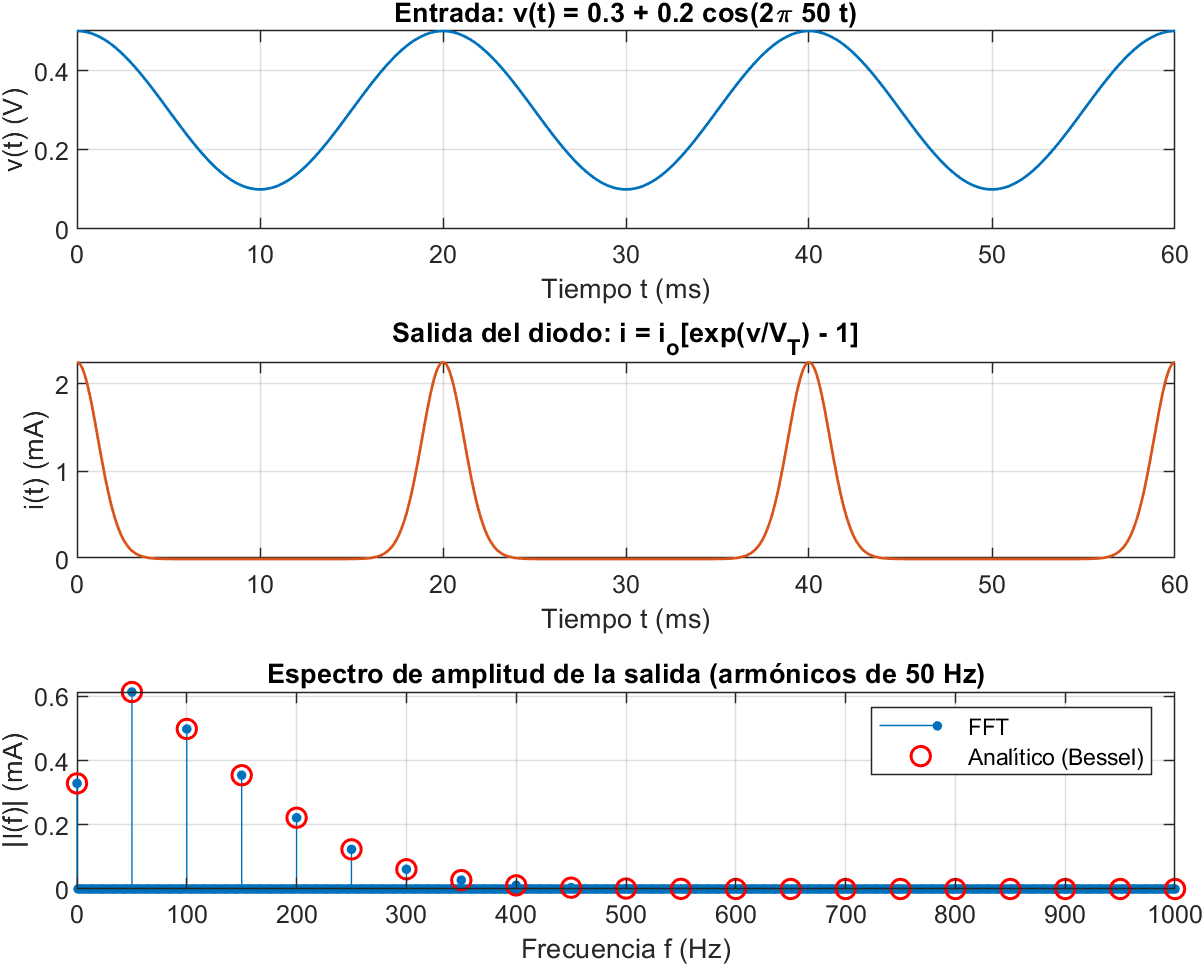
\includegraphics[width=0.95\textwidth]{figuras/punto2b_espectro.png}
\caption{Punto 2b. Arriba: voltaje de entrada. Centro: corriente del diodo, un tren de pulsos
estrechos de \SI{2.25}{mA} de pico, uno por ciclo. Abajo: amplitud del espectro (FFT en azul, solución
de Bessel en rojo).}
\label{fig:2b}
\end{figure}

\begin{figure}[H]
\centering
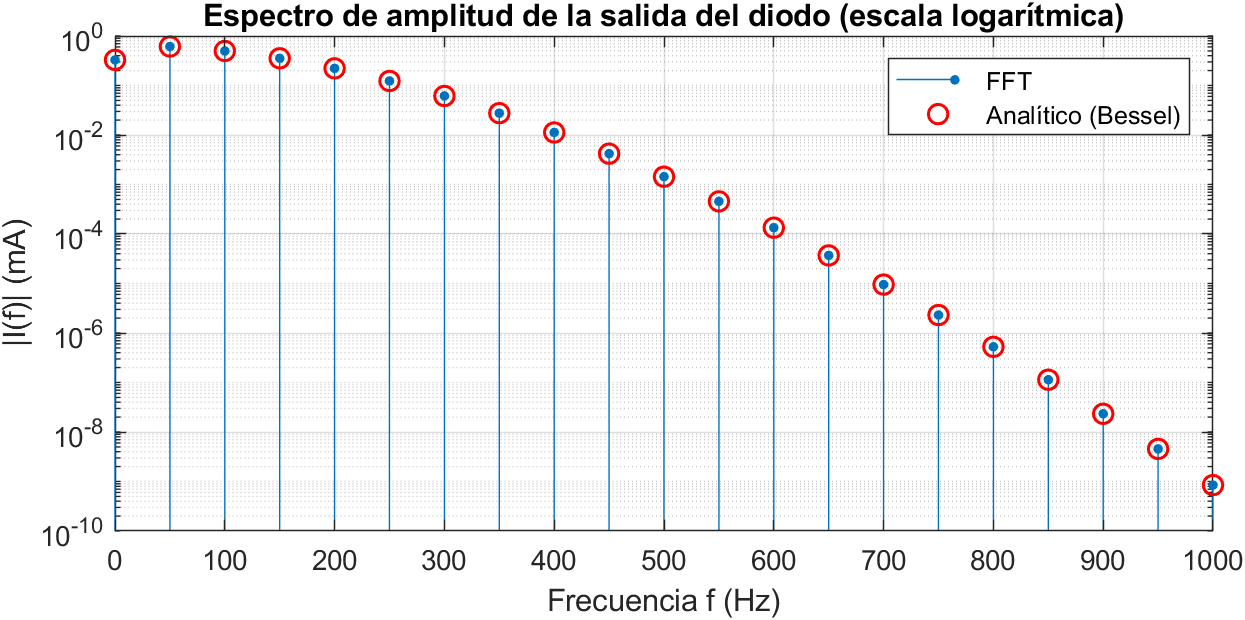
\includegraphics[width=0.95\textwidth]{figuras/punto2b_espectro_log.png}
\caption{Punto 2b en escala logarítmica. La FFT sigue a la solución de Bessel a lo largo de 9 órdenes
de magnitud; los armónicos altos decaen más rápido que una exponencial.}
\label{fig:2blog}
\end{figure}

\textbf{Verificaciones.} Además de la coincidencia línea por línea de la tabla~\ref{tab:2b}:
(1) el promedio temporal de $i(t)$ es \SI{0.329075}{mA}, igual a $A_0$; (2) en $t=0$ todos los
cosenos valen 1, así que $i(0)=\sum_nA_n$: la suma hasta $n=12$ da \SI{2.248058}{mA} y
$i(0)=I_se^x-i_0=\SI{2.248107}{mA}$ (la diferencia es el aporte de $n>12$); (3) el valor RMS calculado
en el tiempo y desde las amplitudes coincide: \SI{0.719990}{mA}.

\textbf{¿Por qué ``mezclador''?} Con una sola frecuencia de entrada la no linealidad solo produce
armónicos y DC. El diodo funciona como mezclador cuando recibe dos tonos $f_1$ y $f_2$ (señal y
oscilador local): la exponencial genera entonces todas las combinaciones $mf_1\pm nf_2$, incluida la
frecuencia intermedia $|f_1-f_2|$, como en el punto 2a pero con infinitos órdenes.

%=====================================================================
\newpage
\section{Punto 3: Razón entre el segundo y tercer armónico por serie de Taylor}
%=====================================================================

\emph{En el problema 2b, estimar la relación de la amplitud entre el segundo y tercer armónico,
considerando el término cuadrado y cúbico en la expansión de serie de Taylor de la función de
transferencia. Compare con los resultados obtenidos en 2b.}

\bigskip

La serie de Taylor de la función de transferencia es el análogo de la expansión de la polarización
en potencias de $\tilde E$: el segundo armónico viene del término cuadrático y el tercero del cúbico.
La señal oscila alrededor de la polarización $V_0$, así que se expande alrededor del punto de
operación. Con $u(t)=v(t)-V_0=V_1\cos\omega t$, como en 2b,
\[
i=I_s\,e^{u/\VT}-i_0,\qquad
e^{u/\VT}=1+\frac{u}{\VT}+\frac{1}{2!}\left(\frac{u}{\VT}\right)^2+\frac{1}{3!}\left(\frac{u}{\VT}\right)^3
+\mathcal O\!\left(\frac{u^4}{\VT^4}\right).
\]
Con $u/\VT=x\cos\omega t$ y linealizando las potencias,
\[
\frac{x^2}{2}\cos^2\omega t=\frac{x^2}{4}+\frac{x^2}{4}\cos2\omega t,\qquad
\frac{x^3}{6}\cos^3\omega t=\frac{x^3}{8}\cos\omega t+\frac{x^3}{24}\cos3\omega t,
\]
y agrupando por frecuencia:
\[
i\approx\underbrace{I_s\left(1+\frac{x^2}{4}\right)-i_0}_{\text{DC}}
+\underbrace{I_s\left(x+\frac{x^3}{8}\right)}_{f}\cos\omega t
+\underbrace{I_s\frac{x^2}{4}}_{2f}\cos2\omega t
+\underbrace{I_s\frac{x^3}{24}}_{3f}\cos3\omega t .
\]
El segundo armónico sale solo del término cuadrático y el tercero solo del cúbico. La razón es
\[
\boxed{\;\frac{A_{2f}}{A_{3f}}\approx\frac{I_sx^2/4}{I_sx^3/24}=\frac6x=\frac{6\VT}{V_1}
=\frac{6(\SI{0.026}{V})}{\SI{0.2}{V}}=0.78\;}
\]
$I_s$ (y con ella $i_0$ y $V_0$) se cancela: la razón solo depende de $V_1/\VT$.

\subsection*{Comparación con el resultado exacto de 2b}

Del punto 2b, $A_n=2I_sI_n(x)$, así que
\[
\left.\frac{A_{2f}}{A_{3f}}\right|_{\text{exacta}}=\frac{I_2(x)}{I_3(x)}=\frac{243.003}{172.775}=1.4065,
\]
que coincide con la razón medida en la FFT (1.4065).

\begin{table}[H]
\centering
\caption{Taylor hasta orden 3 (alrededor de $V_0$) frente al resultado exacto, para $V_1=\SI{0.2}{V}$.}
\label{tab:3}
\begin{tabular}{@{}lccc@{}}
\toprule
Magnitud & Taylor (orden 3) & Exacto (Bessel/FFT) & Taylor/Exacto \\
\midrule
DC (mA)             & 0.0162 & 0.3291 & 0.049 \\
\SI{50}{Hz} (mA)    & 0.0663 & 0.6137 & 0.108 \\
\SI{100}{Hz} (mA)   & 0.0152 & 0.4986 & 0.030 \\
\SI{150}{Hz} (mA)   & 0.0195 & 0.3545 & 0.055 \\
\midrule
Razón $A_{2f}/A_{3f}$ & 0.780 & 1.4065 & 0.555 \\
\bottomrule
\end{tabular}
\end{table}

La serie truncada en orden 3 predice $A_{2f}/A_{3f}=0.78$ frente al valor exacto $1.4065$: subestima
la razón en un 44.5 \%, y las amplitudes absolutas quedan entre 10 y 30 veces por debajo de las reales.
La aproximación no es válida en estas condiciones porque $x=V_1/\VT\approx7.7$ no es pequeño.

\subsection*{¿Por qué falla la aproximación?}

\textbf{1. La serie truncada no representa a la exponencial.} La serie de $e^x$ converge para todo $x$,
pero necesita muchos términos cuando $x$ es grande:
\[
1+x+\frac{x^2}{2}+\frac{x^3}{6}\bigg|_{x=7.69}=114.1\qquad\text{frente a}\qquad e^{7.69}=2191.4 .
\]
Los términos de orden 4, 5, 6, \ldots\ despreciados son mayores que los retenidos ($x^n/n!$ crece
mientras $n<x$ y alcanza su máximo cerca de $n\approx7$), y además también aportan a $2f$ y $3f$:
$\cos^4$ contiene $\cos2\theta$ y $\cos^5$ contiene $\cos3\theta$.

\textbf{2. La razón falla menos que las amplitudes}, porque el error de truncamiento subestima ambos
armónicos y al dividir se cancela en parte.

\textbf{3. Taylor es el límite de señal pequeña del resultado exacto.} Para $x\ll1$ basta el primer
término de la serie de $I_n$, $I_n(x)\approx(x/2)^n/n!$, y
\[
\frac{I_2(x)}{I_3(x)}\approx\frac{(x/2)^2/2!}{(x/2)^3/3!}=\frac{x^2/8}{x^3/48}=\frac6x,
\]
exactamente el resultado de Taylor. Con la siguiente corrección de la serie,
$I_2/I_3\approx(6/x)(1+x^2/48)$, que ya se aparta un 10 \% cuando $x\approx2$. En el extremo opuesto,
$x\gg1$, la aproximación gaussiana del punto 2b da $I_2/I_3\approx e^{(9-4)/(2x)}\to1$, en lugar de
$6/x\to0$.

\begin{figure}[H]
\centering
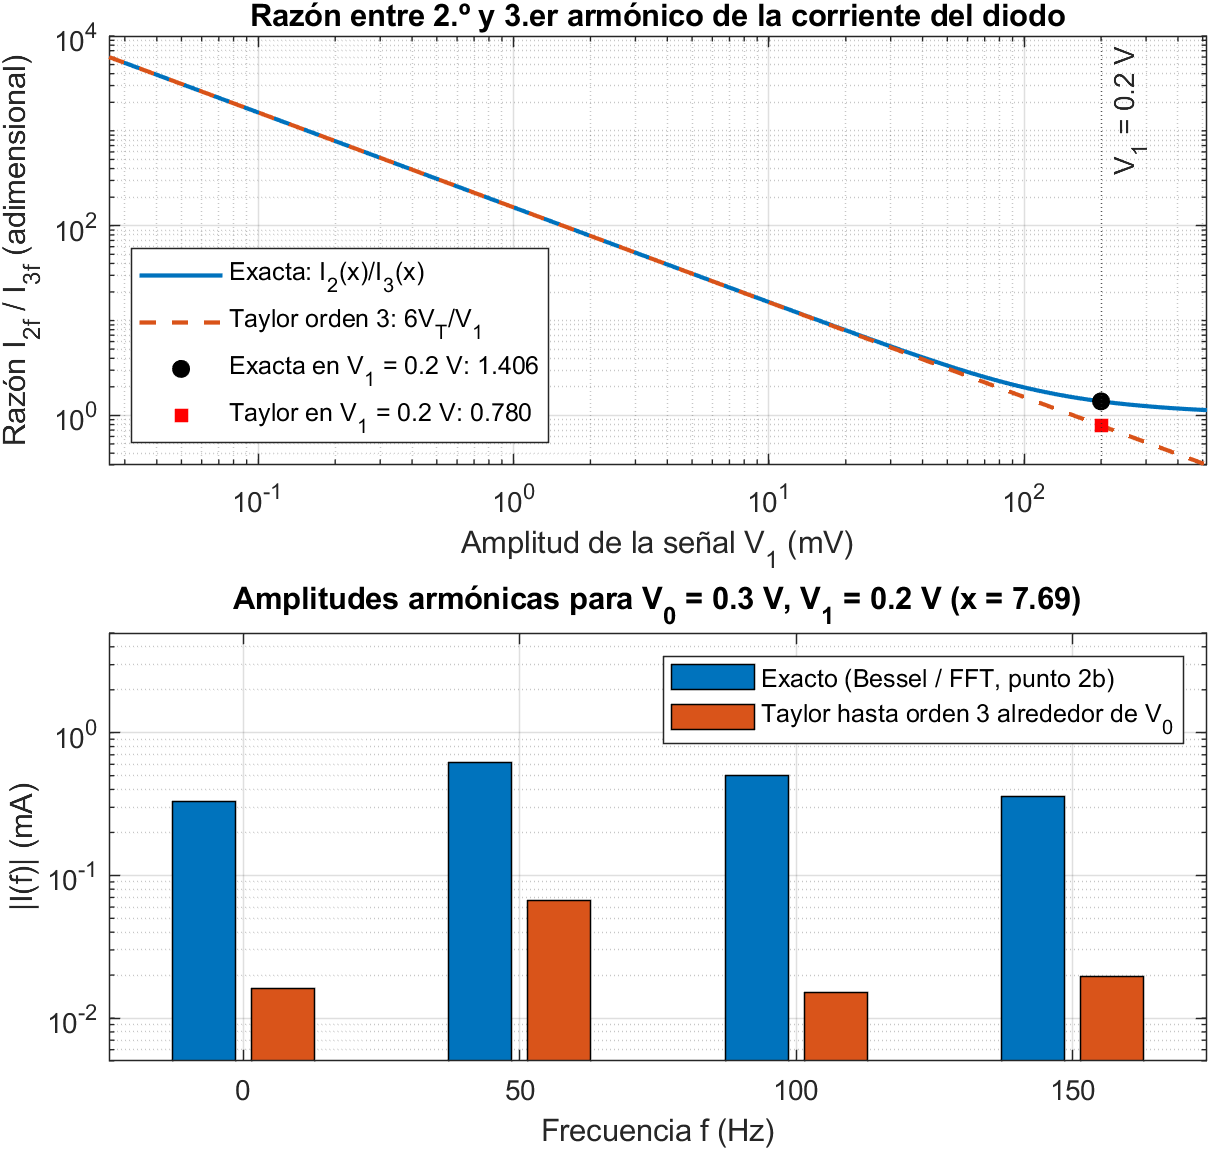
\includegraphics[width=0.92\textwidth]{figuras/punto3_taylor_vs_exacto.png}
\caption{Punto 3. Arriba: razón $A_{2f}/A_{3f}$ en función de la amplitud de la señal $V_1$; la curva
exacta $I_2(x)/I_3(x)$ (azul) y la de Taylor $6V_T/V_1$ (rojo, discontinua) coinciden para señales
pequeñas y se separan cuando $V_1$ llega a unas decenas de mV. Abajo: amplitudes de DC y de los tres
primeros armónicos para $V_1=\SI{0.2}{V}$ (escala logarítmica).}
\label{fig:3}
\end{figure}

\textbf{4. Rango de validez.} Numéricamente (figura~\ref{fig:3}), la estimación $6/x$ tiene un error
menor al 10 \% solo si $x<2.4$, es decir, $V_1<\SI{63}{mV}\approx2.4\,\VT$. Con $V_1=\SI{0.2}{V}$ se
está muy fuera de ese rango.

\subsection*{Variante: expansión alrededor de $v=0$}

Si se expande directamente alrededor de $v=0$,
\[
i\approx i_0\left[\frac{v}{\VT}+\frac{v^2}{2\VT^2}+\frac{v^3}{6\VT^3}\right],\qquad v=V_0+V_1\cos\omega t,
\]
hay que desarrollar las potencias completas:
\begin{align*}
v^2&=V_0^2+2V_0V_1\cos\omega t+V_1^2\cos^2\omega t,\\
v^3&=V_0^3+3V_0^2V_1\cos\omega t+3V_0V_1^2\cos^2\omega t+V_1^3\cos^3\omega t .
\end{align*}
Ahora el término cúbico también aporta al segundo armónico:
\begin{gather*}
A_{2f}=i_0\left[\frac{V_1^2}{4\VT^2}+\frac{3V_0V_1^2}{2\cdot6\VT^3}\right]=\frac{i_0V_1^2}{4\VT^2}\left(1+\frac{V_0}{\VT}\right),
\qquad A_{3f}=\frac{i_0V_1^3}{24\VT^3},\\
\frac{A_{2f}}{A_{3f}}=\frac{6(\VT+V_0)}{V_1}=9.78 .
\end{gather*}
Es mucho peor (casi 7 veces el valor exacto), porque el voltaje llega a \SI{0.5}{V}, unas 19 escalas
térmicas lejos del centro de la expansión. Una serie de potencias debe centrarse en el punto de
operación, y aun así solo sirve si la excursión es pequeña frente a la escala de la no linealidad.

\subsection*{Conexión con la óptica no lineal}

La expansión de $\tilde P$ en potencias de $\tilde E$ también es una serie cuya validez depende de que
el campo aplicado sea pequeño frente a la escala de la no linealidad. En un material esa escala es el
campo atómico, $E_{\text{at}}=e/(4\pi\epsilon_0a_0^2)\approx\SI{5.14e11}{V/m}$, y cada orden está
suprimido aproximadamente por $E/E_{\text{at}}$ (Boyd, p.~3). En el diodo la escala es $\VT$ y
el parámetro de expansión es $V_1/\VT$ (tabla~\ref{tab:analogia}). En óptica, incluso con láseres
intensos, $E/E_{\text{at}}\ll1$ y la expansión perturbativa funciona; en el diodo del problema
$V_1/\VT\approx7.7$, un régimen no perturbativo donde truncar la serie no tiene sentido.

\begin{table}[H]
\centering
\caption{Analogía entre el diodo y un medio óptico no lineal.}
\label{tab:analogia}
\begin{tabular}{@{}lll@{}}
\toprule
& Diodo & Medio óptico \\
\midrule
Entrada & $v(t)$ & $\tilde E(t)$ \\
Respuesta & $i(t)$ & $\tilde P(t)$ \\
Escala de la no linealidad & $\VT=\SI{26}{mV}$ & $E_{\text{at}}\approx\SI{5e11}{V/m}$ \\
Parámetro de expansión & $V_1/\VT$ & $E/E_{\text{at}}$ \\
Segundo armónico & término $u^2$ & $\chi^{(2)}\tilde E^2$ \\
Tercer armónico & término $u^3$ & $\chi^{(3)}\tilde E^3$ \\
\bottomrule
\end{tabular}
\end{table}

%=====================================================================
\newpage
\section{Punto 4: Ejercicios de Saleh y Teich}
%=====================================================================

\emph{Resolver de Saleh y Teich, Fundamentals of Photonics: 5.2-1, 5.3-1, 5.4-1 y
3.1-4.}

\subsection{Ejercicio 5.2-1}

\emph{Dielectric Media. Identify the media described by the following equations, regarding linearity,
dispersiveness, spatial dispersiveness, and homogeneity. Assume that all media are isotropic}
(Saleh y Teich, p.~195). Aquí $\chi$, $a$, $a_1$ y $a_2$ son constantes.

Los criterios son las definiciones de Saleh (§5.2, p.~156): el medio es \emph{lineal} si
$\Pc(\mathbf r,t)$ está relacionado linealmente con $\Ec(\mathbf r,t)$ (vale la superposición);
\emph{no dispersivo} si la respuesta es instantánea, es decir, $\Pc$ en $t$ depende solo de $\Ec$ en ese
mismo $t$; \emph{homogéneo} si la relación entre $\Pc$ y $\Ec$ no depende de la posición $\mathbf r$; y
\emph{espacialmente no dispersivo} si la relación es local, es decir, $\Pc$ en $\mathbf r$ depende solo de
$\Ec$ en ese mismo $\mathbf r$.

\subsubsection*{a) $\Pc=\epsilon_0\chi\Ec-a\nabla\times\Ec$}

\textbf{Linealidad:} completamente lineal, ya que $\Pc$ y $\Ec$ están completamente relacionados por un
operador lineal:
\[
\Pc=\left(\epsilon_0\chi-a\nabla\times\right)\Ec .
\]
El rotacional es lineal, $\nabla\times(c_1\Ec_1+c_2\Ec_2)=c_1\nabla\times\Ec_1+c_2\nabla\times\Ec_2$,
así que se cumple la superposición.

\textbf{Dispersión temporal:} al $\Pc$ depender de $\Ec$ y no estar involucrados operadores temporales
que tengan en cuenta instantes de tiempo anteriores (memoria), implica que el proceso es instantáneo,
completamente no dispersivo temporalmente.

\textbf{Dispersión espacial:} al haber un operador espacial como el rotacional, $\Pc$ no solo depende de
$\Ec$ en $\mathbf r$ sino de valores de $\Ec$ vecinos, por lo que sí hay dependencia espacial; por lo
tanto, dispersión espacial. Con una onda plana, $\Ec=\mathrm{Re}\{\mathbf E_0e^{j\omega t-j\mathbf k\cdot\mathbf r}\}$,
el rotacional se vuelve $\nabla\times\to-j\mathbf k\times$ y
$\mathbf P=\epsilon_0\chi\mathbf E+ja\,\mathbf k\times\mathbf E$: la respuesta depende del vector de onda
$\mathbf k$, igual que la dispersión temporal es una dependencia en $\omega$. Es el modelo de un medio
ópticamente activo (quiral), que Saleh cita como ejemplo de medio espacialmente dispersivo
(Saleh y Teich, p.~156).

\textbf{Homogeneidad:} las constantes involucradas que hablan sobre el material no dependen del
espacio, son completamente constantes, por lo que su sistema es homogéneo.

\subsubsection*{b) $\Pc+a\Pc^2=\epsilon_0\Ec$}

\textbf{Linealidad:} no lineal, ya que el término $a\Pc^2$ hace que $\Pc$ y $\Ec$ no estén relacionados
por un operador lineal. Si $\Ec_1$ produce $\Pc_1$ y $\Ec_2$ produce $\Pc_2$, la suma $\Pc_1+\Pc_2$ no
responde a $\Ec_1+\Ec_2$:
\[
(\Pc_1+\Pc_2)+a(\Pc_1+\Pc_2)^2=\epsilon_0(\Ec_1+\Ec_2)+2a\,\Pc_1\Pc_2\neq\epsilon_0(\Ec_1+\Ec_2),
\]
por el término cruzado $2a\Pc_1\Pc_2$. No se cumple la superposición. Despejando la cuadrática se ve
que $\Pe$ es una función no lineal de $\Ee$,
\[
\Pe=\frac{-1+\sqrt{1+4a\epsilon_0\Ee}}{2a},
\]
que para campos débiles se aproxima a $\Pe\approx\epsilon_0\Ee-a\epsilon_0^2\Ee^2+\cdots$: justamente una
expansión con un término de segundo orden, como en la óptica no lineal.

\textbf{Dispersión temporal:} al $\Pc$ depender de $\Ec$ y no estar involucrados operadores temporales
que tengan en cuenta instantes de tiempo anteriores (memoria), el proceso es instantáneo: la relación
es algebraica y $\Pc(t)$ queda determinado por $\Ec(t)$ en el mismo instante. Es un medio no lineal
sin memoria, $\Pc=\Psi(\Ec)$, como los que describe Saleh (pp.~161--162). Completamente no
dispersivo temporalmente.

\textbf{Dispersión espacial:} no hay operadores espaciales, así que $\Pc$ en $\mathbf r$ solo depende de
$\Ec$ en ese mismo $\mathbf r$. La relación es local: no hay dispersión espacial.

\textbf{Homogeneidad:} la constante $a$ no depende del espacio, por lo que el sistema es homogéneo.

\subsubsection*{c) $a_1\,\partial^2\Pc/\partial t^2+a_2\,\partial\Pc/\partial t+\Pc=\epsilon_0\chi\Ec$}

\textbf{Linealidad:} completamente lineal, ya que $\Pc$ y $\Ec$ están relacionados por un operador
lineal:
\[
\left(a_1\frac{\partial^2}{\partial t^2}+a_2\frac{\partial}{\partial t}+1\right)\Pc=\epsilon_0\chi\,\Ec .
\]
Las derivadas son lineales, así que si $\Ec_1\to\Pc_1$ y $\Ec_2\to\Pc_2$, entonces
$c_1\Ec_1+c_2\Ec_2\to c_1\Pc_1+c_2\Pc_2$.

\textbf{Dispersión temporal:} aquí sí hay operadores temporales. Es la ecuación de un oscilador
armónico forzado y amortiguado (Saleh y Teich, p.~160): para conocer $\Pc(t)$ no basta el valor de $\Ec$
en el instante $t$, hay que resolver la ecuación diferencial con la historia del campo, así que el
medio tiene memoria y es \textbf{dispersivo}. Es el modelo de Lorentz del medio resonante
(Saleh y Teich, ec.~(5.5-15), p.~176), con $a_1=1/\omega_0^2$, $a_2=\sigma/\omega_0^2$ y $\chi=\chi_0$.
Para una onda monocromática, $\partial/\partial t\to j\omega$ y
\[
\left(1-a_1\omega^2+ja_2\omega\right)\mathbf P=\epsilon_0\chi\mathbf E
\quad\Rightarrow\quad
\chi(\omega)=\frac{\chi}{1-a_1\omega^2+ja_2\omega},
\]
una susceptibilidad que depende de la frecuencia (y es compleja, lo que además implica absorción):
eso es la dispersión.

\textbf{Dispersión espacial:} no hay operadores espaciales, así que $\Pc$ en $\mathbf r$ solo depende de
$\Ec$ en ese mismo punto. No hay dispersión espacial.

\textbf{Homogeneidad:} $a_1$, $a_2$ y $\chi$ son constantes que no dependen del espacio, por lo que el
sistema es homogéneo.

\subsubsection*{d) $\Pc=\epsilon_0\{a_1+a_2\exp[-(x^2+y^2)]\}\Ec$}

\textbf{Linealidad:} completamente lineal, ya que $\Pc$ y $\Ec$ están relacionados por un factor
multiplicativo que no depende de $\Ec$: $\Pc=\epsilon_0\chi(\mathbf r)\Ec$ con
$\chi(\mathbf r)=a_1+a_2e^{-(x^2+y^2)}$.

\textbf{Dispersión temporal:} no hay operadores temporales que tengan en cuenta instantes anteriores
(memoria); $\Pc(t)$ depende solo de $\Ec(t)$. Completamente no dispersivo temporalmente.

\textbf{Dispersión espacial:} aunque aparece la posición, no hay operadores espaciales: $\Pc$ en
$\mathbf r$ depende solo de $\Ec$ en ese mismo $\mathbf r$, multiplicado por un factor que cambia de
punto a punto. La relación sigue siendo local, así que no hay dispersión espacial. (No hay que
confundir depender de la posición con depender de los valores vecinos del campo.)

\textbf{Homogeneidad:} aquí las constantes que hablan sobre el material sí dependen del espacio: la
susceptibilidad $\chi(\mathbf r)=a_1+a_2e^{-\rho^2}$, con $\rho^2=x^2+y^2$, cambia con la distancia al
eje $z$. El sistema es \textbf{inhomogéneo} (Saleh y Teich, p.~158). El índice
$n(\rho)=\sqrt{1+a_1+a_2e^{-\rho^2}}$ es máximo en el eje y decrece hacia afuera (si $a_2>0$): es un medio
de índice gradual, como el núcleo de una fibra GRIN.

\begin{table}[H]
\centering
\caption{Resumen del ejercicio 5.2-1 (todos los medios se suponen isótropos).}
\small
\begin{tabular}{@{}lcccc@{}}
\toprule
Medio & Linealidad & \shortstack{Dispersión\\temporal} & \shortstack{Dispersión\\espacial} & Homogeneidad \\
\midrule
a) Rotacional & Lineal & No dispersivo & Dispersivo & Homogéneo \\
b) Término $a\mathcal P^2$ & No lineal & No dispersivo & No dispersivo & Homogéneo \\
c) Oscilador & Lineal & Dispersivo & No dispersivo & Homogéneo \\
d) $\chi(x,y)$ & Lineal & No dispersivo & No dispersivo & Inhomogéneo \\
\bottomrule
\end{tabular}
\end{table}

\subsection{Ejercicio 5.3-1}

\emph{Traveling Standing Wave. The electric-field complex-amplitude vector for a monochromatic wave of
wavelength $\lambda_o$ traveling in free space is $\mathbf E(\mathbf r)=E_0\sin\beta y\,\exp(-j\beta z)\,\xh$.
(a) Determine a relation between $\beta$ and $\lambda_o$. (b) Derive an expression for the magnetic-field
complex-amplitude vector $\mathbf H(\mathbf r)$. (c) Determine the direction of the flow of optical power.
(d) This wave may be regarded as the sum of two TEM plane waves. Determine their directions of
propagation} (Saleh y Teich, p.~195).
\[
\mathbf E(\mathbf r)=E_0\sin(\beta y)\,e^{-j\beta z}\,\xh
\]

\subsubsection*{a) Relación entre $\beta$ y $\lambda_0$}

Si una onda monocromática viaja en espacio libre, no hay dispersión temporal y cada componente del
campo debe cumplir la ecuación de Helmholtz con $k_0=\omega/c_0=2\pi/\lambda_0$
(Saleh y Teich, ec.~(5.3-16), p.~163):
\[
\nabla^2E_x+k_0^2E_x=0 .
\]
Hay que tener cuidado: este campo no es una onda plana, porque además de la fase $e^{-j\beta z}$ tiene
el perfil $\sin(\beta y)$. Por eso $\beta$ no es el número de onda completo sino solo su componente en
$z$. Calculando las derivadas,
\[
\frac{\partial^2E_x}{\partial y^2}=-\beta^2E_x,\qquad
\frac{\partial^2E_x}{\partial z^2}=-\beta^2E_x
\quad\Rightarrow\quad
-\beta^2E_x-\beta^2E_x+k_0^2E_x=0
\]
\[
\Rightarrow\quad 2\beta^2=k_0^2 .
\]
Así:
\[
\boxed{\;\beta=\frac{k_0}{\sqrt2}=\frac{\sqrt2\,\pi}{\lambda_0}\;}
\]
para el caso monocromático. La velocidad de fase a lo largo de $z$ es entonces
$\omega/\beta=\sqrt2\,c_0$, mayor que $c_0$; no hay contradicción, porque la energía no viaja con esa
velocidad (ver el inciso d). El resultado del inciso d confirma este valor.

\subsubsection*{b) Campo magnético}

Para la expresión del campo magnético usamos la ley de Faraday para campos monocromáticos en el
espacio libre (Saleh y Teich, ec.~(5.3-13), p.~163):
\[
\nabla\times\mathbf E=-j\omega\mu_0\mathbf H
\quad\Rightarrow\quad
\mathbf H=\frac{j}{\omega\mu_0}\nabla\times\mathbf E .
\]
Como $E_x$ depende de $y$ y de $z$, el rotacional se calcula completo (el reemplazo
$\nabla\to-j\mathbf k$ solo vale para una onda plana, y aquí el factor $\sin\beta y$ también se deriva):
\[
\nabla\times\mathbf E=
\begin{vmatrix}
\xh & \yh & \zh\\[2pt]
\dfrac{\partial}{\partial x} & \dfrac{\partial}{\partial y} & \dfrac{\partial}{\partial z}\\[8pt]
E_x(\mathbf r) & 0 & 0
\end{vmatrix}
=\frac{\partial E_x}{\partial z}\,\yh-\frac{\partial E_x}{\partial y}\,\zh
\]
\[
=-j\beta E_0\sin(\beta y)e^{-j\beta z}\,\yh-\beta E_0\cos(\beta y)e^{-j\beta z}\,\zh .
\]
Multiplicando por $j/(\omega\mu_0)$:
\[
\mathbf H=\frac{\beta E_0}{\omega\mu_0}\left[\sin(\beta y)\,\yh-j\cos(\beta y)\,\zh\right]e^{-j\beta z}.
\]
Con $\beta=k_0/\sqrt2$ y $k_0/(\omega\mu_0)=1/(c_0\mu_0)=1/\eta_0$:
\[
\boxed{\;\mathbf H(\mathbf r)=\frac{E_0}{\sqrt2\,\eta_0}\left[\sin(\beta y)\,\yh-j\cos(\beta y)\,\zh\right]e^{-j\beta z}\;}
\]
A diferencia de una onda plana, $\mathbf H$ tiene una componente longitudinal $H_z$ (en cuadratura, por
el factor $-j$). Se verifica que $\nabla\cdot\mathbf H=0$:
\begin{align*}
\frac{\partial H_y}{\partial y}+\frac{\partial H_z}{\partial z}
&=\frac{E_0}{\sqrt2\,\eta_0}\left[\beta\cos\beta y-j\cos\beta y\,(-j\beta)\right]e^{-j\beta z}\\
&=\frac{E_0}{\sqrt2\,\eta_0}\left[\beta\cos\beta y-\beta\cos\beta y\right]e^{-j\beta z}=0 .
\end{align*}
Y la otra ecuación de Maxwell, $\nabla\times\mathbf H=j\omega\epsilon_0\mathbf E$, se cumple
precisamente porque $2\beta^2=k_0^2$.

\subsubsection*{c) Dirección del flujo de potencia óptica}

La dirección de la potencia óptica se halla calculando el vector de Poynting complejo,
$\mathbf S=\tfrac12\mathbf E\times\mathbf H^*$, cuya parte real da el flujo promedio de potencia
(Saleh y Teich, ecs.~(5.3-9)--(5.3-10), p.~163). Como $\mathbf E$ solo tiene componente $x$,
\[
\mathbf S=\tfrac12E_x\left(\xh\times H_y^*\yh+\xh\times H_z^*\zh\right)
=\tfrac12\left(E_xH_y^*\,\zh-E_xH_z^*\,\yh\right),
\]
\[
\mathbf S=\frac{|E_0|^2}{2\sqrt2\,\eta_0}\left[\sin^2(\beta y)\,\zh-j\sin(\beta y)\cos(\beta y)\,\yh\right].
\]
La componente en $\yh$ es imaginaria pura (potencia reactiva, que va y vuelve sin transporte neto), así
que
\[
\boxed{\;\mathrm{Re}\{\mathbf S\}=\frac{|E_0|^2}{2\sqrt2\,\eta_0}\sin^2(\beta y)\,\zh\;}
\]
Por lo tanto, la energía se dirige en dirección $\zh$, al igual que la fase espacial. La intensidad
$I(y)=|E_0|^2\sin^2(\beta y)/(2\sqrt2\,\eta_0)$ forma franjas en $y$ (nula en $y=m\pi/\beta$): en $y$ la onda
es estacionaria y en $z$ es viajera, de ahí el nombre ``traveling standing wave''.

\subsubsection*{d) Descomposición en dos ondas planas TEM}

\[
\mathbf E(\mathbf r)=E_0\sin(\beta y)\,e^{-j\beta z}\,\xh
\]
Usando la relación de Euler $\sin(\beta y)=\frac{1}{2j}\left(e^{j\beta y}-e^{-j\beta y}\right)$:
\[
\mathbf E(\mathbf r)=\frac{E_0}{2j}\left(e^{j\beta y}-e^{-j\beta y}\right)e^{-j\beta z}\,\xh
=\frac{E_0}{2j}\Big[\underbrace{e^{-j\beta(-y+z)}}_{\text{onda 1}}-\underbrace{e^{-j\beta(y+z)}}_{\text{onda 2}}\Big]\xh .
\]
Cada término tiene la forma $e^{-j\mathbf k\cdot\mathbf r}$ de una onda plana (Saleh y Teich, ec.~(5.4-2), p.~165):
\begin{align*}
\text{Onda 1: }&\mathbf k_1=\beta(0,-1,1),\quad\text{dirección }\boxed{(0,-1,1)}\,;\\
\text{Onda 2: }&\mathbf k_2=\beta(0,1,1),\quad\text{dirección }\boxed{(0,1,1)}\,.
\end{align*}
Normalizando, las direcciones son $(0,\mp1,1)/\sqrt2$: ambas están en el plano $y$--$z$, a $\pm45^\circ$
del eje $z$. Las dos son TEM, porque el campo $\xh$ es perpendicular a ambos $\mathbf k$. Su suma se
propaga en promedio en $+z$ (inciso c) y su interferencia en $y$ produce el patrón $\sin(\beta y)$.
Además, cada onda plana en el espacio libre debe tener $|\mathbf k|=k_0$, y
$|\mathbf k_{1,2}|=\sqrt2\,\beta=k_0$, lo que confirma el resultado del inciso a.

\subsection{Ejercicio 5.4-1}

\emph{Electric Field of Focused Light. (a) 1 W of optical power is focused uniformly on a flat target of
size $0.1\times0.1$ mm$^2$ placed in free space. Determine the peak value of the electric field $E_0$
(V/m). Assume that the optical wave is approximated as a TEM plane wave within the area of the target.
(b) Determine the electric field at the center of a Gaussian beam (a point on the beam axis at the beam
waist) if the beam power is 1 W and the beam waist radius $W_0=0.1$ mm. Refer to Sec.~3.1}
(Saleh y Teich, p.~195).

\subsubsection*{a) Potencia enfocada uniformemente}

Para una potencia óptica de \SI{1}{W} enfocada en un área de $0.1\times0.1$ mm$^2$ se tiene una
intensidad óptica de
\[
I=\frac{\SI{1}{W}}{\SI{0.01}{mm^2}}=\SI{100}{W/mm^2}=\SI{1e8}{W/m^2}.
\]
Y sabemos que la intensidad sale del módulo cuadrado del campo eléctrico con la siguiente fórmula
(Saleh y Teich, ec.~(5.4-8), p.~166):
\[
I=\frac{|E_0|^2}{2\eta_0}=\frac12c_0\epsilon_0E_0^2 ,
\]
donde se usó $1/\eta_0=\sqrt{\epsilon_0/\mu_0}=c_0\epsilon_0$. Como se trata de una irradiación
uniforme, no hay un punto específico en el cual debamos medir el valor pico del campo eléctrico: es el
mismo en todo el blanco.
\begin{align*}
E_0&=\sqrt{\frac{2I}{c_0\epsilon_0}}=\sqrt{\frac{2\,(\SI{1e8}{W/m^2})}{(\SI{2.998e8}{m/s})(\SI{8.854e-12}{F/m})}}\\
&\approx\boxed{\SI{2.745e5}{V/m}}\ (\approx\SI{274492}{V/m}).
\end{align*}

\subsubsection*{b) Haz gaussiano}

Para el caso de una distribución de intensidad gaussiana (ya no uniforme), el pico de intensidad se
localiza en el centro del haz. La intensidad es (Saleh y Teich, ec.~(3.1-12), p.~77)
\[
I(\rho,z)=I_0\left[\frac{W_0}{W(z)}\right]^2e^{-\frac{2\rho^2}{W^2(z)}}.
\]
Para $z$ en el punto de enfoque (la cintura), $W(0)=W_0=\SI{0.1}{mm}$:
\[
I(\rho)=I_0\,e^{-\frac{2\rho^2}{W_0^2}}.
\]
Integrando sobre todo el plano deberíamos obtener una potencia óptica de \SI{1}{W}
(Saleh y Teich, ec.~(3.1-14), p.~78):
\begin{align*}
\SI{1}{W}&=\int_0^{2\pi}\!\!\int_0^{\infty}I_0\,e^{-\frac{2\rho^2}{W_0^2}}\rho\dd\rho\dd\phi\\
&=2\pi I_0\frac{W_0^2}{-4}\int_0^{\infty}\left(-\frac{4\rho}{W_0^2}\right)e^{-\frac{2\rho^2}{W_0^2}}\dd\rho\\
&=\frac{2\pi I_0W_0^2}{-4}\,e^{-\frac{2\rho^2}{W_0^2}}\bigg|_0^{\infty}
=\frac{2\pi}{4}I_0W_0^2 ,
\end{align*}
que es la ecuación (3.1-15) de Saleh, $P=\tfrac12I_0(\pi W_0^2)$. Despejando,
\[
I_0=\frac{2P}{\pi W_0^2}=\frac{2\,(\SI{1}{W})}{\pi(\SI{1e-4}{m})^2}\approx\SI{6.366e7}{W/m^2}\approx\SI{63.66}{W/mm^2}.
\]
Así, para el pico se tendrá una intensidad de $I_0\approx\SI{63.66}{W/mm^2}$. Aplicando la misma fórmula
para el campo eléctrico, se tiene
\begin{align*}
E_0&=\sqrt{\frac{2I_0}{c_0\epsilon_0}}=\sqrt{\frac{2\,(\SI{6.366e7}{W/m^2})}{(\SI{2.998e8}{m/s})(\SI{8.854e-12}{F/m})}}\\
&\approx\boxed{\SI{2.190e5}{V/m}}\ (\approx\SI{219013}{V/m}).
\end{align*}
El pico del haz gaussiano es menor que el campo del caso uniforme porque el área efectiva del haz,
$\pi W_0^2/2\approx\SI{0.0157}{mm^2}$, es mayor que la del blanco de \SI{0.01}{mm^2}.

\subsection{Ejercicio 3.1-4}

\emph{Determination of the Width and Curvature at One Point Given the Width and Curvature at Another
Point. Assume that the width and radius of curvature of a Gaussian beam of wavelength $\lambda=1\ \mu$m at
some point on the beam axis are $W_1=1$ mm and $R_1=1$ m, respectively. Determine the beam width $W_2$ and
radius of curvature $R_2$ at a distance $d=10$ cm to the right} (Saleh y Teich, p.~84).

\bigskip

Parámetros: $\lambda=\SI{1}{\micro m}$, $W_1=\SI{1}{mm}$, $R_1=\SI{1}{m}$, $d=\SI{10}{cm}$.

Para determinar el ancho y el radio para cualquier distancia $z$ se usan sus respectivas fórmulas
(Saleh y Teich, ecs.~(3.1-8), (3.1-9) y (3.1-11), p.~77):
\[
W(z)=W_0\sqrt{1+\left(\frac{z}{z_0}\right)^2},\qquad
R(z)=z\left[1+\left(\frac{z_0}{z}\right)^2\right],\qquad
W_0=\sqrt{\frac{\lambda z_0}{\pi}},
\]
con $z_0$ la distancia de Rayleigh. Para un $z_1$ tenemos un $W_1$ y un $R_1$, medido desde la posición
de $W_0$:
\[
W_1=W_0\sqrt{1+\left(\frac{z_1}{z_0}\right)^2},\qquad
R_1=z_1\left[1+\left(\frac{z_0}{z_1}\right)^2\right],\qquad\text{con }z_0=\frac{\pi W_0^2}{\lambda}.
\]
Reemplazando $z_0$:
\[
W_1^2=W_0^2\left[1+\left(\frac{z_1\lambda}{\pi W_0^2}\right)^2\right],\qquad
R_1=z_1\left[1+\left(\frac{\pi W_0^2}{\lambda z_1}\right)^2\right].
\]
De las dos ecuaciones se despeja el mismo término:
\[
\left(\frac{W_1^2}{W_0^2}-1\right)^{-1}=\left(\frac{\pi W_0^2}{\lambda z_1}\right)^2,\qquad
\frac{R_1}{z_1}-1=\left(\frac{\pi W_0^2}{\lambda z_1}\right)^2 .
\]
Igualando,
\[
\frac{1}{\frac{W_1^2}{W_0^2}-1}+1=\frac{R_1}{z_1}
\quad\Rightarrow\quad
\frac{\cancel{1}+\frac{W_1^2}{W_0^2}-\cancel{1}}{\frac{W_1^2}{W_0^2}-1}
=\frac{(W_1/W_0)^2}{(W_1/W_0)^2-1}=\frac{R_1}{z_1},
\]
\[
\Rightarrow\quad z_1=R_1\,\frac{(W_1/W_0)^2-1}{(W_1/W_0)^2}=R_1\left[1-\left(\frac{W_0}{W_1}\right)^2\right].
\]
Reemplazando $z_1$ en $W_1^2=W_0^2\left[1+\left(\frac{z_1\lambda}{\pi W_0^2}\right)^2\right]$ y usando
software para encontrar las soluciones para $W_0$ (script \texttt{punto4\_cintura\_haz.py}),
obtenemos
\[
W_0\approx\SI{0.3033}{mm},\qquad z_1\approx\SI{0.908}{m},\qquad z_0=\frac{\pi W_0^2}{\lambda}\approx\SI{0.289}{m}.
\]
La ecuación también tiene la raíz trivial $W_0=W_1$, que se descarta porque da $z_1=0$ (el plano de la
cintura, donde $R=\infty\neq\SI{1}{m}$). La raíz no trivial se puede escribir en forma cerrada: con
$u=(W_0/W_1)^2$ y $b=\lambda R_1/(\pi W_1^2)=0.3183$ la ecuación queda $u(1-u)=b^2(1-u)^2$, cuya raíz no
trivial es $u=b^2/(1+b^2)$, es decir,
\[
W_0=\frac{W_1}{\sqrt{1+\left(\pi W_1^2/\lambda R_1\right)^2}},\qquad
z_1=\frac{R_1}{1+\left(\lambda R_1/\pi W_1^2\right)^2},
\]
que son las ecuaciones (3.1-26) y (3.1-25) de Saleh (p.~84) y dan los mismos valores.
Con este resultado podemos hallar, para la distancia extra $d=\SI{10}{cm}$, el nuevo ancho y radio. Así:
\[
W_2=W_0\sqrt{1+\left(\frac{(z_1+d)\lambda}{\pi W_0^2}\right)^2}\approx\boxed{\SI{1.100}{mm}},
\]
\[
R_2=(z_1+d)\left[1+\left(\frac{\pi W_0^2}{\lambda(z_1+d)}\right)^2\right]\approx\boxed{\SI{1.091}{m}}.
\]
(Con los valores sin redondear, $W_2=\SI{1.1005}{mm}$ y $R_2=\SI{1.0909}{m}$.) El haz sigue abriéndose
al alejarse de la cintura: $z_1$ y $z_1+d$ están a unas 3 distancias de Rayleigh, en la región donde
$W(z)$ crece casi linealmente (figura~\ref{fig:haz}).

\begin{figure}[H]
\centering
\begin{tikzpicture}
\begin{axis}[
  width=0.85\textwidth, height=5.5cm,
  xlabel={Distancia a la cintura, $z$ (m)}, ylabel={Ancho del haz, $W(z)$ (mm)},
  xmin=-0.05, xmax=1.3, ymin=0, ymax=1.5, domain=-0.05:1.3, samples=200,
  axis lines=left, grid=major, grid style={black!10},
  label style={font=\small}, tick label style={font=\footnotesize}]
  \addplot[blue!60!black, thick] {0.303314*sqrt(1+(x/0.289025)^2)};
  \addplot[only marks, mark=*, red!75!black] coordinates {(0.908,1.0) (1.008,1.1005)};
  \addplot[only marks, mark=o, black] coordinates {(0,0.303314)};
  \node[font=\footnotesize, anchor=west] at (axis cs:0.32,0.18) {$W_0=0.303$ mm};
  \node[font=\footnotesize, anchor=south east] at (axis cs:0.9,1.02) {$(z_1,W_1)$};
  \node[font=\footnotesize, anchor=north west] at (axis cs:1.02,1.08) {$(z_1+d,W_2)$};
  \draw[dashed, black!50] (axis cs:0.289,0) -- (axis cs:0.289,0.429) node[above, font=\footnotesize, black] {$z_0$};
\end{axis}
\end{tikzpicture}
\caption{Ejercicio 3.1-4: ancho del haz gaussiano en función de la distancia a la cintura, con
$\lambda=\SI{1}{\micro m}$, $W_0=\SI{0.303}{mm}$ y $z_0=\SI{0.289}{m}$. Se marcan el punto dado
$(z_1,W_1)$ y el punto pedido $(z_1+d,W_2)$.}
\label{fig:haz}
\end{figure}

\end{document}
